\documentclass[a4paper,12pt]{article}
\usepackage{cmap}
\usepackage[T1,T2A]{fontenc}  % кодировка
\usepackage[utf8]{inputenc}   % кодировка исходного текста
\usepackage[english,russian]{babel} % локализация и переносы
\usepackage{geometry}
\usepackage{titling}
\usepackage{minted}
\usepackage{graphics}
\usepackage{graphicx}

\renewcommand\maketitlehooka{\null\mbox{}\vfill}
\renewcommand\maketitlehookd{\vfill\null}

% геометрия
\geometry{pdftex, left = 2cm, right = 2cm, top = 2.5cm, bottom = 2.5cm}
\setcounter{tocdepth}{4} % фикс переноса 
\righthyphenmin = 2
\tolerance = 2048

% заголовок
\title{Отчет по Лабораторной работе №8\\[150mm]}
\author{Чепиго Дарья \\ИУ7-44Б}
\date{}

\begin{document}
	\begin{titlepage}
		\maketitle
		\thispagestyle{empty}
	\end{titlepage}
	
	\newpage
	\noindent\textbf{Условие задачи:}

	Реализация и исследование отсечения отрезка регулярным отсекателем алгоритмом Кируса-Бека.\\
	
	\noindent\textbf{Этапы работы программы:}
	\begin{enumerate} 
		\item Ввод отсекателя
		\item Ввод произвольных отрезков (не одного, а нескольких) - можно сделать мышкой, но клавиатурный ввод должен быть
		\item Выполнение отсечения: границы отсекателя показать одним цветом, отрезок -- другим, результат отсечения -- третьим.
	\end{enumerate}
	
	\noindent\textbf{Алгоритм Кируса-Бека:}
	
	Отметим форму, в которой описываются отрезки в данном алгоритме (параметрическая форма задания отрезка):
	
	\[P(t) = P1 + (P2  - P1) * t\]
%	где t - параметр $(0 <= t <= 1)$.\\
	
	Это векторное уравнение, которое в двумерной графике можно свести к двум одномерным параметрическим уравнениям следующего вида:
	
	\[Px(t) = P1.x + (P2.x  - P1.x) * t\]
	%\[Py(t) = P1.y+ (P2.y  - P1.y) * t\]
	параметр t так же принадлежит [0, 1]\\
	
	Если значение параметра t лежит вне [0, 1], то пересечение происходит с продолжением отрезка (получается, что его нет). Такие пересечения отвергаются.\\
	
	\textit{Вектор внутренней нормали} $n\_v$ - вектор, перпендикулярный грани многоугольника и направлен внутрь этого многоугольника. Это проверяется аналитическим выражением следующего вида: \[n\_v * (B - A) >= 0\]
	где А - точка грани, из которой исходит данная нормаль, а В любая другая точка нормали (следует брать точку, не принадлежащую рассматриваемой грани, иначе скалярное произведение будет равно 0.)\\
	
	Следующий вектор: \[[P(t) - f\_i]\]
	где $f\_i$ - произвольная точка рассматриваемой грани (не совпадающая с точкой пересечения рассматриваемых грани и отрезка)
	\newpage
	
	Проанализируем скалярное произведение этого вектора и вектора нормали к рассматриваемой грани:\\
	
	$n\_v * [P(t) - f\_i] > 0$ - вектор направлен внутрь области многоугольника (из скалярного произведения следует, что угол между вектором и вектором внутренней нормали < 90).\\
	
	$n\_v * [P(t) - f\_i] = 0$ - вектор перпендикулярен нормали (то есть параллелен грани)\\
	
	$n\_v * [P(t) - fif\_i] < 0$ - направлен вне области многоугольника (противоположность первой ситуации)\\
	
	В зависимости t, рассматриваемая точка P(t) может находиться как внутри, так и вне области многоугольника относительно рассматриваемой грани, однако в данном случае нас больше интересует тот факт, что мы можем определить <<входит>> или <<выходит>> отрезок из многоугольника при пересечении определенной грани.\\
	
	Если отрезок пересекает грань и его начало было внутри многоугольника относительно этой грани, то получается что при пересекании он выйдет за грань и за пределы многоугольника.\\
	
	Рассмотрим подробнее ситуацию: 	\[n\_v*[P(t) - f\_i] = 0\] 
	когда вектор, состоящий из точки отрезка P(t) и точки  f\_i грани параллелен этой грани. Очевидно, что если стоит задача построить параллельную прямую к некоторой прямой L через точку А, находящейся на этой прямой L, то решение этой задачи - прямая, совпадающая с прямой L. Из этого следует, что 	$n\_v*[P(t) - fi] = 0$ выполняется тогда, когда вектор лежит на одной прямой с гранью $[P(t) - fi]$, а P(t) для некоторого t - точка пересечения грани и отрезка.\\
	
	Подставим параметрическую форму уравнения в данное выражение:
	
	\[n\_v * [P1 + (P2  - P1)t - f\_i] = 0\]
	
	Преобразуем:  	\[n\_v * [P1 - f\_i] + 	n\_v * [P2  - P1]t  = 0\]     \\           
	
	В данном уравнении вектор $[P2  - P1]$ - вектор, определяющий направление (ориентацию) отрезка, а вектор $[P1 - f\_i]$  рассматривался выше в общем виде, но в данном случае - вектор, соединяющий некоторую точку грани с началом отрезка (по его скалярному произведению с внутренней нормалью можно судить о положении отрезка относительно внутренней нормали)\\
	
	Введем обозначения:\\
	\[Wi = n\_v[P1 - f\_i]\]
	\[Dск = n\_v[P2  - P1]\]
	
	Выразим t из уравнения (*), используя обозначения выше:
	\[t = -Wi / Dск\]
	
	Данное выражение нельзя рассматривать при Dск = 0.\\

	Рассмотрим случаи, когда Dск = 0:
	
	\begin{enumerate} 
		\item Вектор ориентации отрезка вырожден (нулевой). Такой случай нас не очень интересует.
		\item Dcк перпендикулярен n\_v. Получается, что отрезок парллелен грани. Здесь может быть 2 случая: 
		\begin{enumerate} 
			\item отрезок лежит вне многоугольника относительно грани - он однозначно  не видим. Заканчиваем операцию отсечения данного отрезка. 
			\item  Отрезок лежит внутри многоугольника относительно грани - тогда следует перейти на следующую итерацию и продолжить операцию отсечения. 
		\end{enumerate}
	
		Определить "вне" или "внутри" легко с помощью вектора Wi. Этот вектор начинается в некоторой точке рассматриваемой грани многоугольника и заканчивается в некоторой точке отрезка. Можно сказать, что он направлен "от грани к отрезку". Внутренняя нормаль начинается в некоторой точке грани и может быть направлена к отрезку и в противоположную сторону. 
		Проверяется это, например, вот таким скалярным произведением: 
		\[Wi = n\_v[P1 - f\_i]\] 
		Если скалярное произведение < 0, то угол между вектором нормали и вектором, направленным к отрезку > 90, и вектор лежит вне фигуры, иначе - внутри. 
	
	\end{enumerate}

	
	Осталось решить только одну проблему: какие конкретно значения t выбрать в качестве начального и конечного. Очевидно, что если отрезок виден, то он виден относительно всех граней. Из этого можно сделать вывод, что если отрезок входит в многоугольник относительно какой-то грани, то относительно других граней он должен был уже войти (то есть надо выбирать в качестве начала последний вход), и при этом не должен был выйти (то есть получается последний вход должен быть раньше всех выходов).\\
	
	С выходами ситуация та же: выйдя за первую грань, отрезок перестанет быть виден относительно нее и, следовательно, будет на оставшемся промежутке (из этого вывод - в качестве конца следует брать первых выход).\\
	
	Далее, убедившись, что параметр tвх , соответствующий последнему входу, меньше, чем параметр tвых, соответствующий первому выходу, чертим видимую часть отрезка (если условие не выполняется - не чертим).
	\newpage
	\noindent\textbf{Алгоритм с комментариями из моей программы (файл main.py):}
	
	
	\begin{minted}[fontsize=\footnotesize]{python3}
	def cut_one(line: QLine, count):
	# Вычисление директрисы заданного отрезка:
	# D = P_2-P_1
	d = QPointF(line.x2() - line.x1(), line.y2() - line.y1())
	
	# Инициализация пределов значений параметра t при условии,
	# что отрезок полностью видим:
	top = 0
	bottom = 1
	
	# Начало цикла по всем сторонам отсекателя.
	# Для каждой i-ой стороны отсекателя выполнить следующие действия:
	for i in range(-2, count - 2):
	# Вычисление вектора внутренней нормали к очередной i-ой стороне отсекателя - N_вi
		norm = normal(wind.cutter[i], wind.cutter[i + 1], wind.cutter[i + 2])
	
		# Вычисление вектора W_i=P_1-f_i (f_i берем за вершины стороны)
		w = QPointF(line.x1() - wind.cutter[i].x(), line.y1() - wind.cutter[i].y())
	
		# Вычисление скалярного произведения векторов:
		# W_iскал=W_i N_вi, D_скал=DN_вi
		d_scal = scalar_mult(d, norm)
		w_scal = scalar_mult(w, norm)
		
		# Если D_скал=0, Если W_скi>0, то отрезок
		# (точка) видим(-а) относительно текущей стороны отсекателя
		if d_scal == 0:
			if w_scal < 0:
				return []
			else:
				continue
	
		# Вычисление параметра t:
		t = -w_scal / d_scal
	
		if d_scal > 0:
			if t <= 1:
				top = max(top, t)
			else:
				return
		elif d_scal < 0:
			if t >= 0:
				bottom = min(bottom, t)
			else:
				return
	
	
		# Проверка фактической видимости отсечённого отрезка. Если t_н > t_в, то выход
		if top > bottom:
			break
	
	# Проверка фактической видимости отсечённого отрезка.
	# Если t_н<=t_в, то изобразить отрезок в  интервале от P(t_н ) до P(t_в ).
	if top <= bottom:
		return QLine(round(line.x1() + d.x() * top), round(line.y1() + d.y() * top),
		round(line.x1() + d.x() * bottom), round(line.y1() + d.y() * bottom))
	\end{minted}
	
	
	\newpage
	\noindent\textbf{Интерфейс и примеры работы:}\\\\
	Главное окно:\\\\
	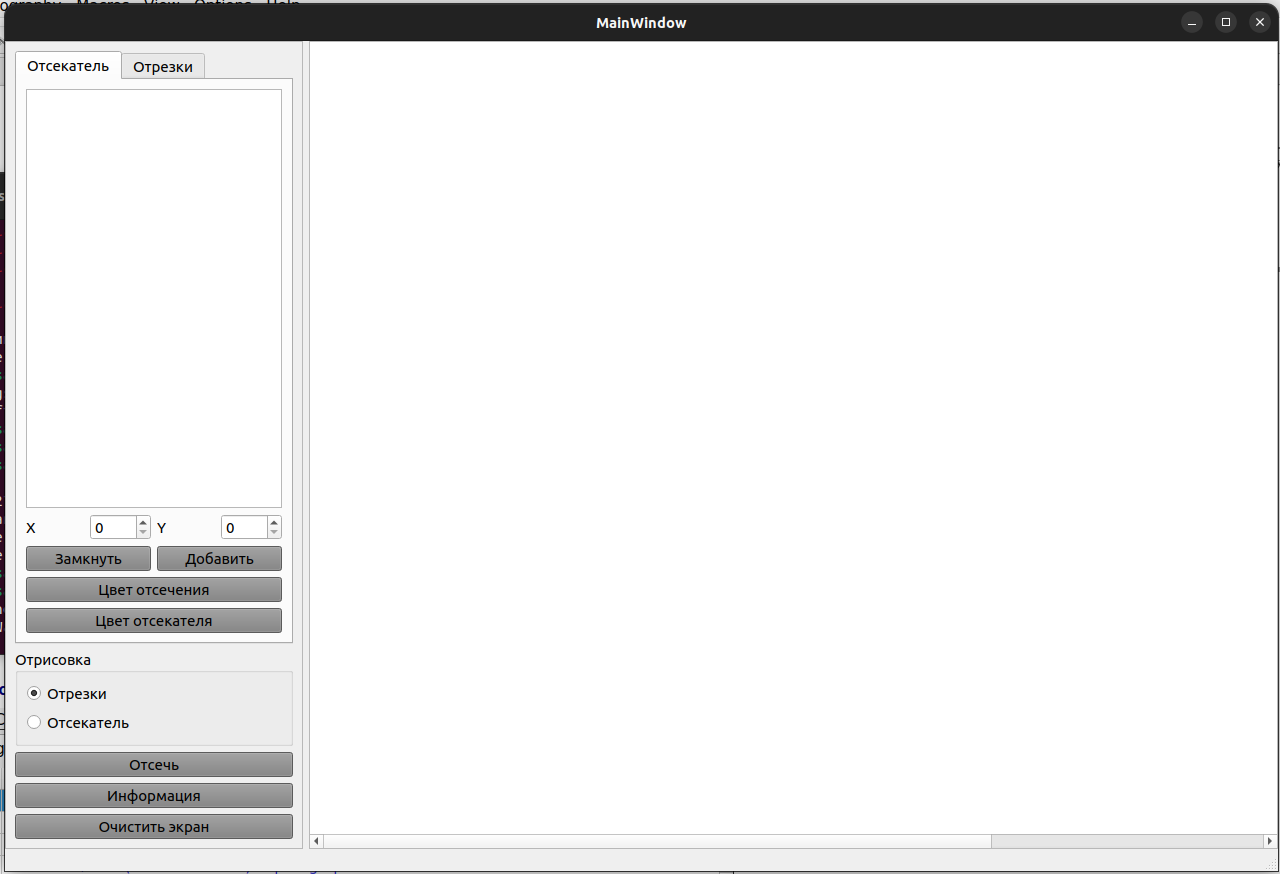
\includegraphics[width=\linewidth]{mainwindow}\\\\
	Информация о программе:\\\\
	
\includegraphics[width=\linewidth]{infor}
	\newpage
	\noindent Попробуем задать невыпуклый отсекатель:\\\\
	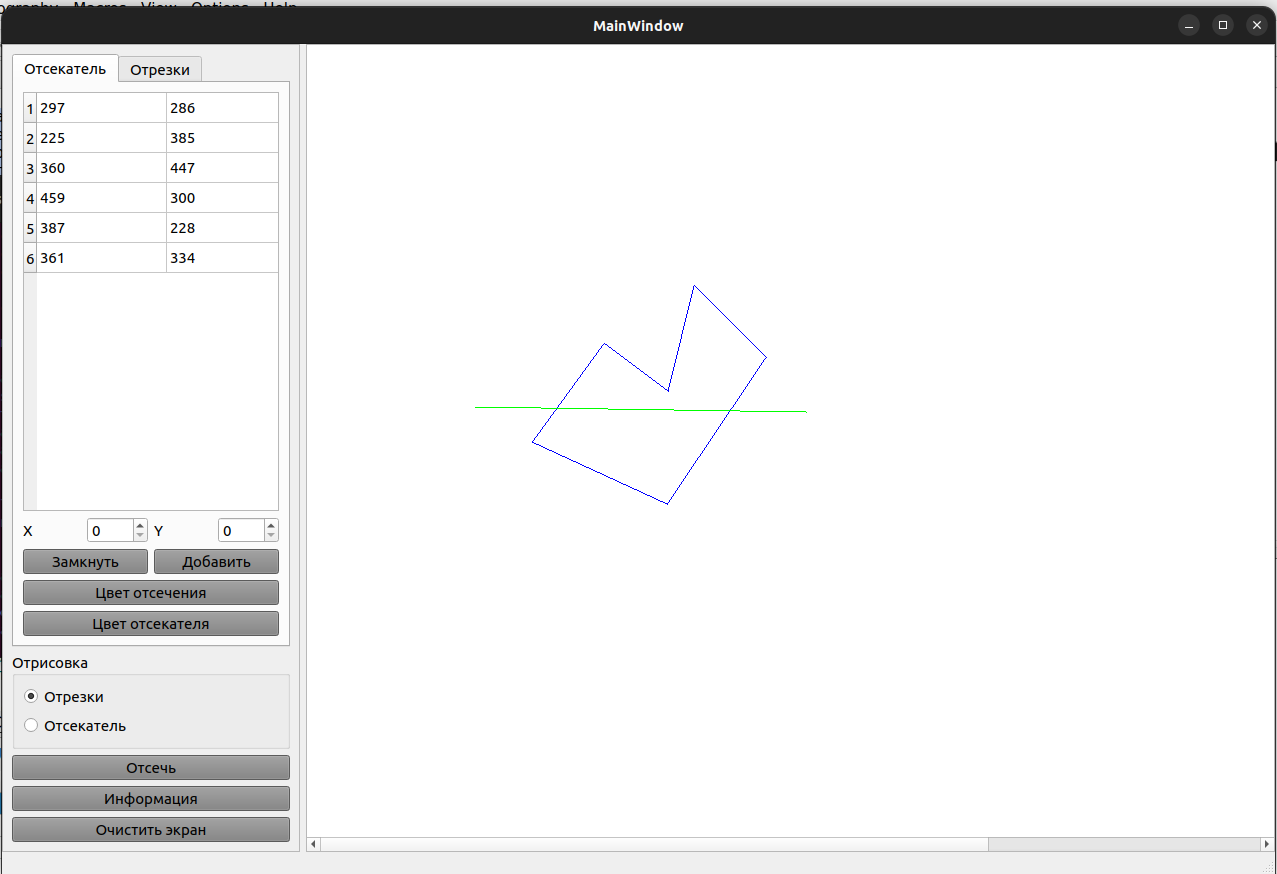
\includegraphics[width=\linewidth]{errorpol}\\\\
	отсекаем:\\\\
	
\includegraphics[width=\linewidth]{error}
	\newpage
	Зададим выпуклый отсекатель и отрезки, выберем цвет отсекаемых отрезков:\\\\
	
\includegraphics[width=\linewidth]{color}\\
	отсекаем:\\\\
	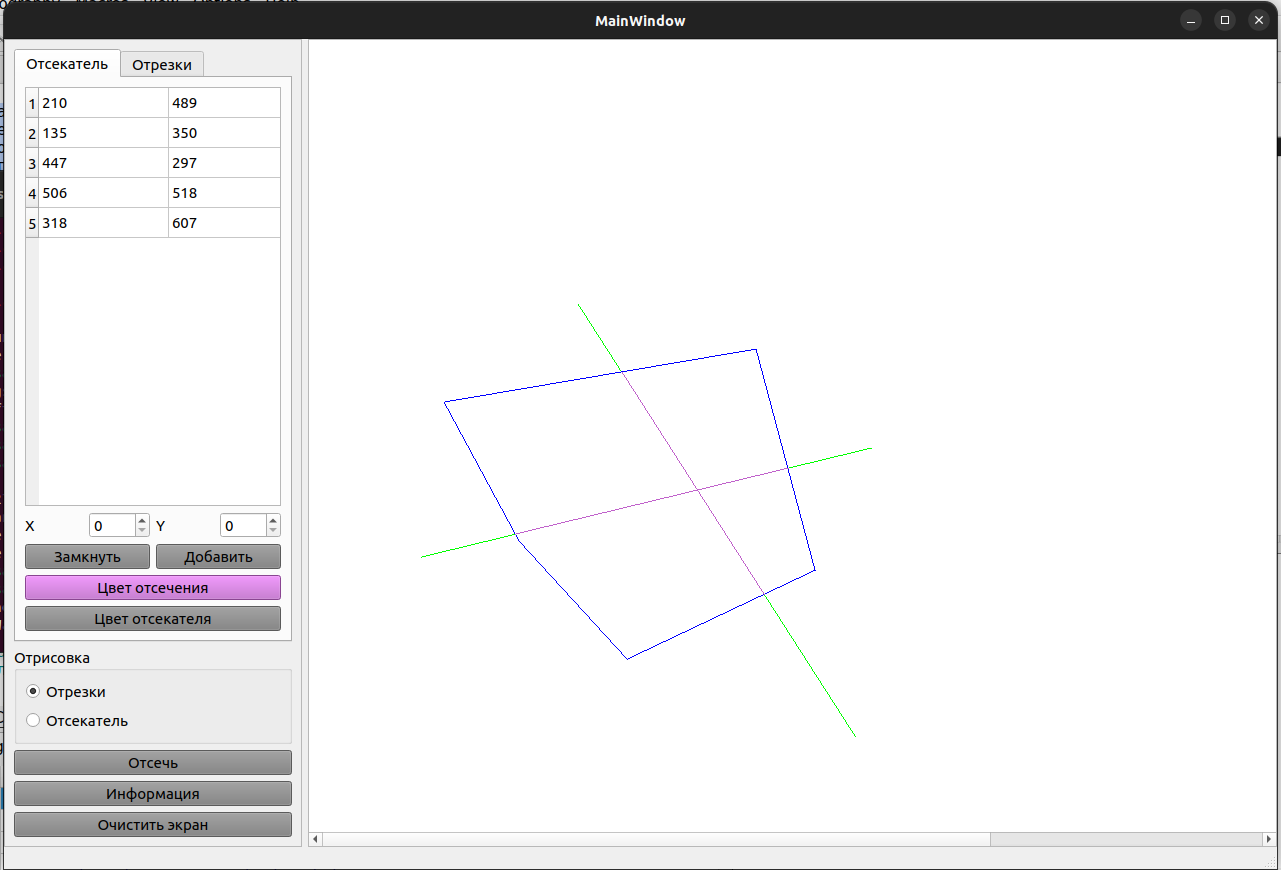
\includegraphics[width=\linewidth]{normal}
	

\end{document}